% Un articolo scritto con LaTeX
\documentclass[a4paper,11pt]{article}
\usepackage{graphicx}
\usepackage[T1]{fontenc} % codifica dei font in uscita
\usepackage[utf8]{inputenc} % lettere accentate da tastiera
\usepackage[italian]{babel} % lingua principale del documento
\usepackage{url}
\usepackage [a4paper, top=2.5cm, bottom=2.5cm, left=1.5cm, right=1.5cm, bindingoffset=8mm] {geometry}

% inizio documento
             
\begin{document}

\begin{center}



\textsc{\Huge Esperienza IV}\\[0.5cm]



\large
\title{ESPERIENZA IV}

Michele \textsc{Pedrotti}\\
Luigi \textsc{Bassini}\\
Nicola \textsc{Trevisson}\\
Giacomo \textsc{Alberini}






\end{center}

%\tableofcontents

~\\
%\textbf{Introduzione}\\\\
\section{Scopo dell'esperienza}
Lo scopo di questa esperienza è quello di tarare una valvola a spillo. Una valvola a spillo ( o \textit{Fine control needle valve}), è un particolare tipo di valvola che permette di conoscere il flusso di gas in entrata, e risulta estremamente importante in determinati contesti. Il nostro obiettivo sarà proprio quello di misurare il flusso in entrata in una camera di volume (misurato come variazione di pressione in funzione del tempo), al variare del numero di giri di apertura della valvola.


\section{Taratura della valvola a spillo}
\subsection{Impianto da vuoto}
Per misurare il flusso di gas in entrata nella camera, e quindi tarare la valvola a spillo, è necessario creare il vuoto nella camera. Per raggiungere questo scopo si è utilizzato l'impianto da vuoto già descritto nella relazione precedente. Ne riportiamo di seguito uno schema:
\vspace{-10 pt} 
 \begin{center} 
\begin{figure}[htpd]
\hspace{20 pt}
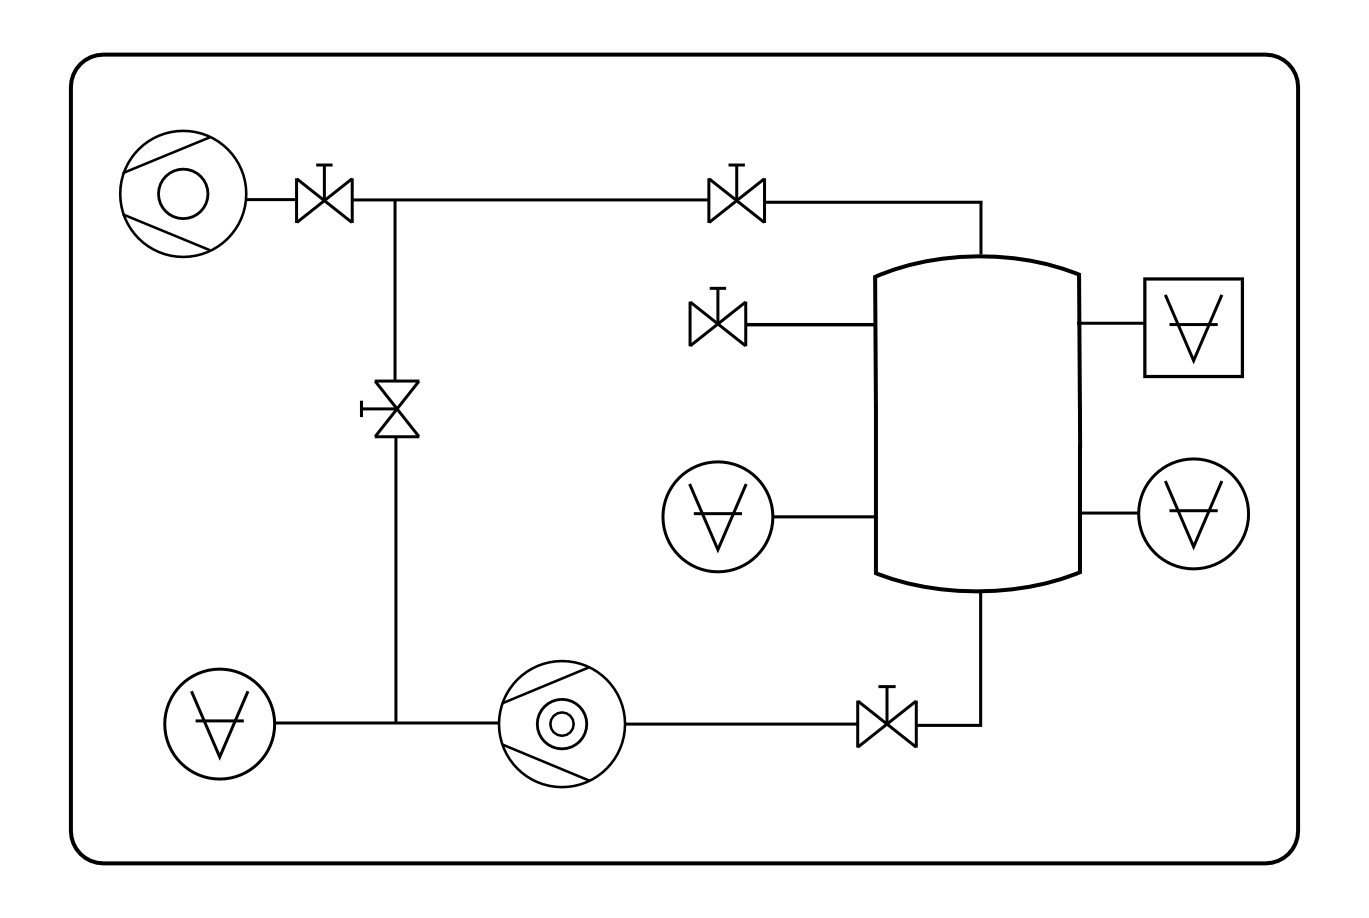
\includegraphics[scale=0.4]{schema_finale.png}


\end{figure}
\end{center}

Per prima cosa abbiamo misurato il flusso di gas dovuto alle perdite dell'impianto. Questo flusso dovrà successeivamente essere sottratto alle misure di flusso relative alla valvola a spillo. Per questa prima misura abbiamo raggiunto il vuoto limite del nostro impianto (circa $1.2\cdot10^{-5}$ mbar), e abbiamo quindi misurato la pressione in funzione del tempo utilizzando il software in nostra dotazione.
Successivamente abbiamo creato nuovamente il vuoto limite nella camera (utilizzando le precauzioni dovute in modo da non danneggiare la pompa turbomolecolare). Durante questo processo abbiamo tenuto completamente aperti i due rubinetti della valvola a spillo (tappando ovviamente l'uscita così da non provocare un repentino riflusso di gas all'interno della camera), così da evitare che si creasse un volume morto nella valvola che avrebbe poi pesantemente inciso sui primi dati acquisiti. Raggiunto il vuoto limite abbiamo sigillato la camera (tenendo accesa la pompa turbomolecolare),calibrato la valvola a spillo sulla prima tacca e quindi tolto il tappo all'uscita della valvola. Con il software abbiamo quindi acquisito i dati Pressione-Tempo. 
A questo proposito è rilevante notare che le misure acquisite in entrata dal software sono relative al voltaggio attraverasante il Pirani. Questo comporta due importanti situazioni. Prima di tutto il range del Pirani va da $10^{-3}$ mbar a 10 mbar, quindi le misure di pressioni inferiori o superiori a questi valori non possono essere considerate attendibili. Inoltre il Pirani lavora attraverso diverse conversioni, e per questo l'incertezza sulle misure di pressione è molto elevata, dell'ordine del 5\%\ in termini di errore relativo. 
Una volta acquisiti i dati è necessario ripetere l'intera sequenza aprendo  la volvola alla seconda tacca. L'operazione è stata ripetuta otto volte, fino ad aprire la valvola all'ottava tacca.  
Una volta acquisiti i dati sperimentali, abbiamo graficato l'andamento della pressione in funzione del tempo. Si può notare che questo andamento è di tipo lineare. Riportiamo nel grafico seguente la rappresentazione del quarto set di dati:
 \begin{center} 
\begin{figure}[htpd]
\hspace{-50 pt}
\includegraphics{graficoP4.png}


\end{figure}
\end{center}


Questo andamento è analogo a tutti gli altri set di dati, cioè del tipo: $Y=a+bX$, dove Y è la pressione e X il tempo. Tramite regressione lineare abbiamo quindi calcolato i parametri a e b, e verificato la bontà del fit tramite test del chi quadro. Riportiamo nella seguente tabella i risultati ottenuti:\\
\vspace{10 px}\\

\hspace{-30 pt}
\begin{tabular}{|c|c|c|c|c|c|}
\hline $Tacche$ & $a\pm$$\delta a$ [Pa] & $b\pm$$\delta b$ [$s^{-1}$] & $\chi^{2}\ped{sperimentale}$ & $\chi^{2}\ped{teorico}$ & $Q\pm\delta Q$ [$pa\cdot m^{3}$$\cdot s{-1}$] \\ 
\hline 1 & 1.84$\cdot10^{-2}$$\pm 0.05\cdot10^{-2}$ &  36.7$\cdot10^{-5}$$\pm 0.06\cdot10^{-5}$ & 2896 & 2801 & -1.88$\cdot10^{-7}$$\pm 0.07\cdot10^{-7}$ \\ 
\hline 2 & 3$\cdot10^{-4}$$\pm 1\cdot10^{-4}$ & 29.04$\cdot10^{-4}$$\pm 0.08\cdot10^{-4}$ & 238 & 683 & 1.480$\cdot10^{-5}$$\pm 5\cdot10^{-8}$ \\ 
\hline 3 & -2.4$\cdot10^{-2}$$\pm 0.1\cdot10^{-2}$ &  2.80$\cdot10^{-3}$$\pm 0.01\cdot10^{-3}$ & 192 & 456 & 1.415$\cdot10^{-5}$$\pm 7\cdot10^{-8}$ \\ 
\hline 4 & -2.8$\cdot10^{-2}$$\pm 0.2\cdot10^{-2}$ &  5.41$\cdot10^{-3}$$\pm 0.03\cdot10^{-3}$ & 81 & 214 & 2.97$\cdot10^{-5}$$\pm 2\cdot10^{-7}$ \\ 
\hline 5 & -1.91$\cdot10^{-1}$$\pm 0.04\cdot10^{-1}$ & 3.51$\cdot10^{-2}$$\pm 0.01\cdot10^{-2}$ & 95 & 202 & 2.06$\cdot10^{-5}$$\pm 9\cdot10^{-7}$ \\ 
\hline 6 & -1.98$\pm 0.03$  & 5.36$\cdot10^{-1}$$\pm 0.02\cdot10^{-1}$ & 104 & 177 & 3.18$\cdot10^{-3}$$\pm 1\cdot10^{-5}$ \\ 
\hline 7 & -33.1$\pm 0.12$ & 8.32$\pm 0.03$ & 103 & 194 & 4.93$\cdot10^{-2}$$\pm 2\cdot10^{-4}$ \\ 
\hline 8 & -1107$\pm 3$ & 50.5$\pm 0.1$  & 915 & 325 & 3.00$\cdot10^{-1}$$\pm 1\cdot10^{-3}$ \\ 
\hline 
\end{tabular} \\
\\
\\


Nella tabella compare anche il parametro Q. Q è il flusso di aria entrante nella camera di volume ed è misurato come:
$Q=V\cdot \frac{dP}{dt}-Q0$, dove V è 5930$\pm 30$ $cm^{3}$,  $\frac{dP}{dt}$ è il parametro b precedentemente stimato, e $Q0 =2.365\cdot10^{-6}\pm 5\cdot10^{-9}$ il flusso dovuto alle perdite dell'impianto da vuoto.  Notiamo che il primo valore di flusso ha valore negativo. Questo si può spiegare col fatto che il flusso dovuto all'apertura di una tacca della valvola a spillo ha valore infinitesimo, e che il flusso dovuto alle perdite dell'impianto non è costante nel tempo. E' quindi plausibile che il flusso di fondo fosse diverso dal valore Q0 da noi misurato al momento dell'acquisizione dei dati relativi alla prima tacca, e che questo abbia prodotto un risultato negativo. Inseriamo di seguito il grafico relativo al flusso Q in funzione del numero di giri della valvola a spillo:
 \begin{center} 
\begin{figure}[htpd]
\hspace{-57.5pt}
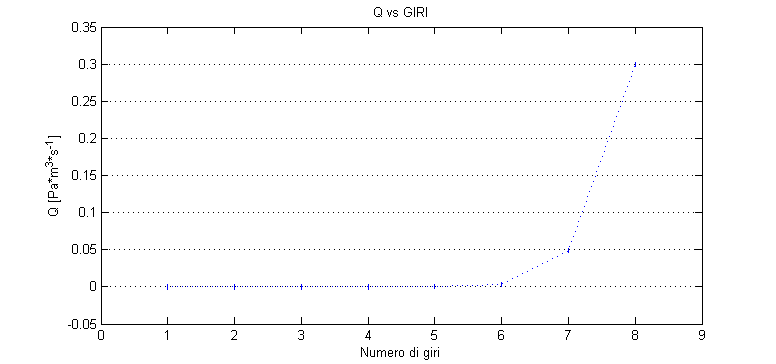
\includegraphics{graficoQ.png}
\end{figure}
\end{center}
Si nota subito che i primi cinque valori di flusso non possono essere distinti nella definizione del grafico. Al contrario, a partire dal sesto giro della valvola a spillo, il flusso aumenta in maniera esponenziale. Il flusso in funzione dei giri della valvola sembra quindi avere una relazione del tipo: $Q=a\cdot exp(b\cdot G)$ dove G è il numero di giri della valvola a spillo.  
Abbiamo quindi proceduto nel calcolare i parametri del fit ottenendo i seguenti risultati:

\begin{center}

\begin{tabular}{|c|c|c|c|}
\hline $a$ [$Pa\cdot \frac{m^{3}}{s}$] & $\delta a$ [$Pa\cdot \frac{m^{3}}{s}$] & $b$ & $\delta b$ \\ 
\hline  $1.2\cdot 10^{-7}$ & $0.1\cdot 10^{-7}$ & 1.8 & 0.2 \\ 
\hline 
\end{tabular}
 
\end{center}
\end{document} 